
\documentclass[9pt,a4paper,twocolumn,twoside]{tau-class/tau}
\usepackage[english]{babel}

\journalname{Babeș-Bolyai University, Faculty of Mathematics and Computer Science}
\title{Software Engineering Laboratory Report - Team 922/1}

%----------------------------------------------------------
% AUTHORS, AFFILIATIONS AND PROFESSOR
%----------------------------------------------------------
\author[1]{Team Leaders: Bogdan Borodi}
\author[1]{Rareș-Andrei Cotoi}

%----------------------------------------------------------

\affil[1]{2nd Year, Group 922/1}

%----------------------------------------------------------
% FOOTER INFORMATION
%----------------------------------------------------------

\institution{Babeș-Bolyai University, Faculty of Mathematics and Computer Science}
\footinfo{Laboratory Report 922/1}
\theday{April 29, 2025}
\leadauthor{Rareș Cotoi and Bogdan Borodi}
\course{Software Engineering 2024-2025}

% %----------------------------------------------------------
% % ABSTRACT AND KEYWORDS
% %----------------------------------------------------------

% \begin{abstract}    
%     Welcome to tau ($\tau$) \LaTeX\ class designed especially for your lab reports or academic articles. In this example template, we will guide you through the process of using and customizing this document to your needs. For more information of this class check out the appendix section. There, you will find codes that define key aspects of the template, allowing you to explore and modify them.
% \end{abstract}

%----------------------------------------------------------

%----------------------------------------------------------

\begin{document}
		
    \maketitle 
    \thispagestyle{firststyle} 
    % \tableofcontents
    % \linenumbers 
    
%----------------------------------------------------------

\section{Introduction}
Our team was formed by merging teams "Steampunks" and "Vlad și ardelenii" and hence the Team Leaders splitted as following: Rareș Cotoi (TL of Steampunks) - \textit{Team Lead} and Bogdan Borodi (TL of Vlad și ardelenii) - \textit{Technical Lead}. As for the team members, the final team is being formed by the students: Bota Mihnea, Chiș Denis, Cotîrlă Darius, Radu Cioată, Andrei Cruceru, Teodora Buga, Cezar Chiticariu, Tudor Buha, Vlad Cenușe and Robert Bota.

\section{Task breakdown and distribution}
The tasks from Assignment 4 were broken down into smaller tasks and splitted among all the team members by Rareș Cotoi and Bogdan Borodi. All the tasks were created and monitored using GitHub issues and projects, having a board created and associated to our main repository.
\begin{figure}[H]
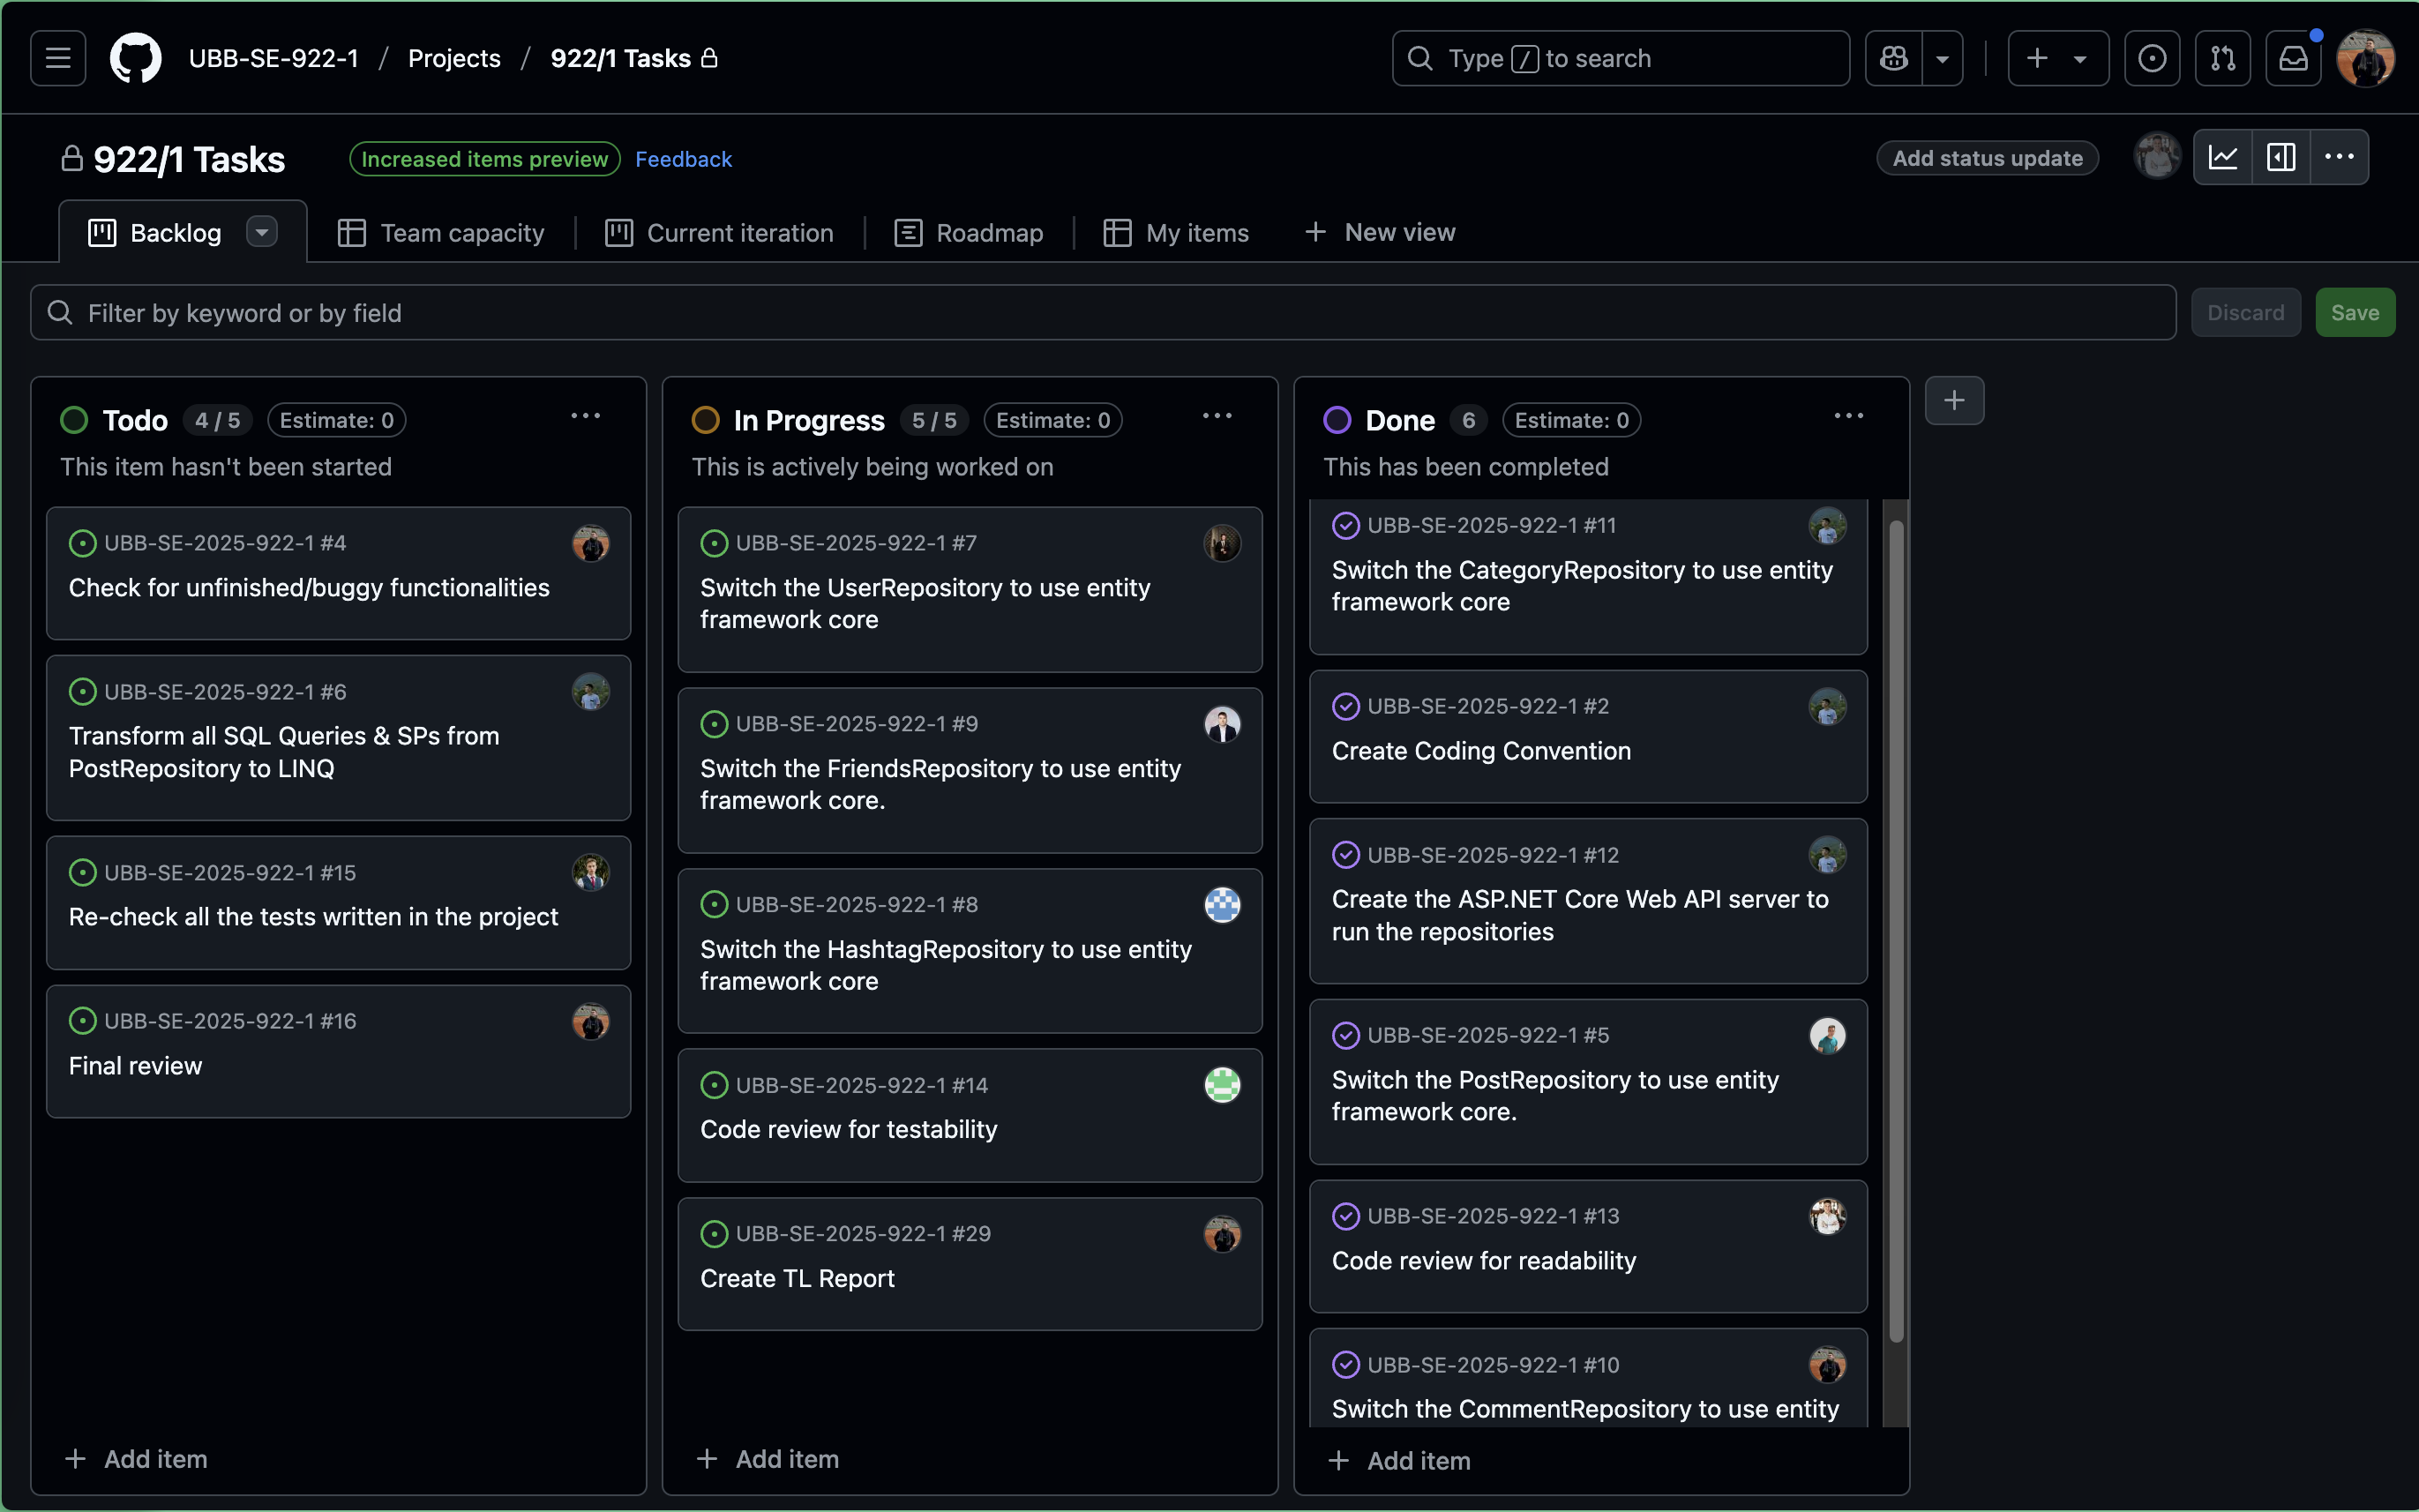
\includegraphics[width=0.9\columnwidth]{backlog.png}
\centering
\caption{Sample from our tasks board}
\end{figure}
The tasks were splitted based on every feature that we implemented, as following:
\subsection{Merging projects}
\begin{itemize}
    \item Check and resolve mock functions and features in both applications to merge: \textit{Vlad Cenușe};
    \item Resolve merge conflicts: \textit{Bogdan Borodi}; 
    \item Check for potential business logic in the UI or Data Access Layer: \textit{Vlad Cenușe, Tudor Buha};
    \item Final code review for merging projects: \textit{Bogdan Borodi, Rareș Cotoi};
\end{itemize}

\subsection{Switch the repository side to use entity framework core}
For this task, the existing Repositories were handled individually as following:
\begin{itemize}
    \item Category Repository: \textit{Bogdan Borodi};
    \item Comment Repository: \textit{Rareș Cotoi}; 
    \item Post Repository: \textit{Vlad Cenușe};
    \item User Repository: \textit{Tudor Buha};
    \item Friends Repository: \textit{Denis Chiș} and \textit{Teodora Buga};
    \item Hashtag Repository: \textit{Robert Bota};
\end{itemize}
For all repositories migration mentioned above, the code review was done by \textit{Bogdan Borodi}.

\subsection{Setup the ASP.NET Core Web API Server to run the Repository}
For this part, initially, the server was configured by \textit{Bogdan Borodi}. After the initial configuration, each Repository was modified to establish a direct connection to the Server, instead of connecting directly to the Database. Each repository was handled by:
\begin{itemize}
    \item Category Repository: \textit{Bogdan Borodi};
    \item Comment Repository: \textit{Rareș Cotoi}; 
    \item Post Repository: \textit{Vlad Cenușe};
    \item User Repository: \textit{Tudor Buha};
    \item Friends Repository: \textit{Denis Chiș} and \textit{Radu Cioată};
    \item Hashtag Repository: \textit{Robert Bota};
\end{itemize}
For this part, the code review was done by \textit{Bogdan Borodi}.

\subsection{Additional tasks}
In addition to the previous tasks categories, some individual and necessary tasks were handled by the team members, as following:
\begin{itemize}
    \item Failing tests fixing - some of the tests we had on the Repository side were failing due to the migration to the Server side: handled by \textit{Bota Mihnea} and \textit{Darius Cotîrlă};
    \item Creating the coding convention: \textit{Bogdan Borodi}; 
    \item Global code review for readability: \textit{Radu Cioată};
    \item Global code review for testability: \textit{Teodora Buga};
    \item Check for unfinished/buggy functionalities: \textit{Rareș Cotoi} and \textit{Bogdan Borodi};
\end{itemize}

\section{Code contribution for each team member}
Having this tasks breakdown, in the dedicated GitHub Repository were made \textbf{47} different commits, using  \textbf{13} different branches:
\begin{itemize}
    \item Branch \textbf{Bob/MergeProjects} - 3 commits, authored by \textit{Bogdan Borodi}:
    \begin{figure}[H]
    \includegraphics[width=0.9\columnwidth]{Bob:MergeProjects.png}
    \centering
    \caption{Branch "Bob/MergeProjects"}
    \end{figure}
    \item Branch \textbf{Bob/MovingToServer} - 4 commits, authored by \textit{Bogdan Borodi}:
    \begin{figure}[H]
    \includegraphics[width=0.9\columnwidth]{Bob:MovingToServer.png}
    \centering
    \caption{Branch "Bob/MovingToServer"}
    \end{figure}
    \item Branch \textbf{Bob/RefactorProject} - 3 commits, authored by \textit{Bogdan Borodi}:
    \begin{figure}[H]
    \includegraphics[width=0.9\columnwidth]{Bob:RefactorProject.png}
    \centering
    \caption{Branch "Bob/RefactorProject"}
    \end{figure}
    \item Branch \textbf{Bob/StyleConventionDocument} - 1 commit, authored by \textit{Bogdan Borodi}:
    \begin{figure}[H]
    \includegraphics[width=0.9\columnwidth]{Bob:StyleConventionDocument.png}
    \centering
    \caption{Branch "Bob/StyleConventionDocument"}
    \end{figure}
    \item Branch \textbf{ChisuFriends} - 7 commits, authored by \textit{Bogdan Borodi} and \textit{Denis Chiș}:
    \begin{figure}[H]
    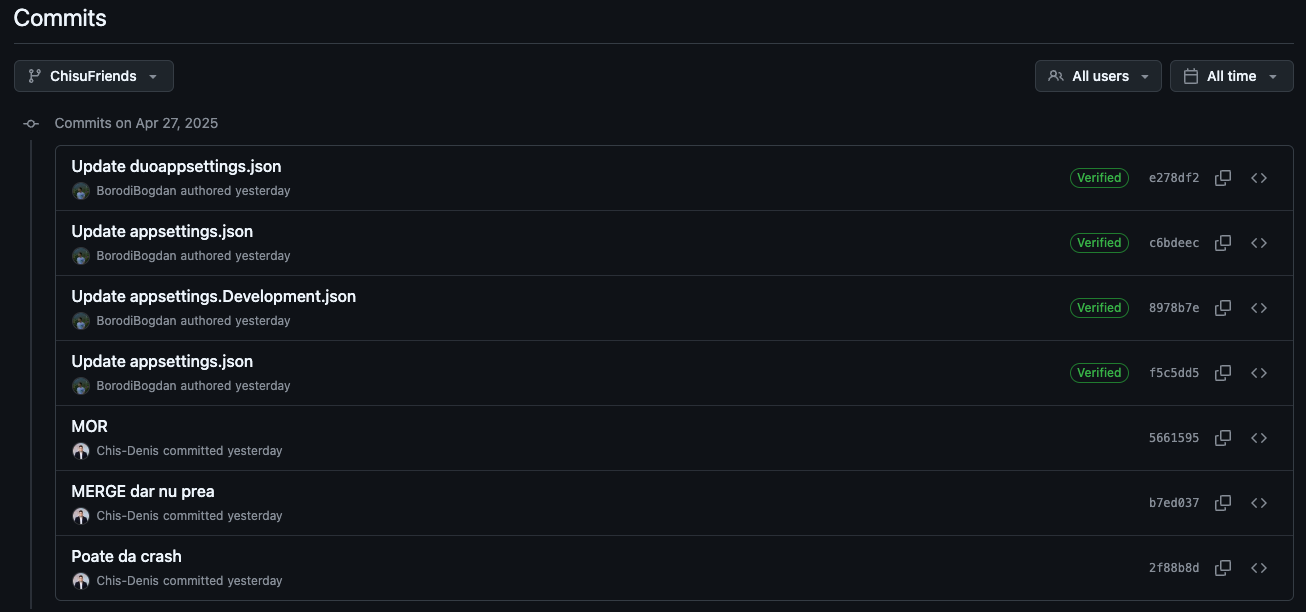
\includegraphics[width=0.9\columnwidth]{ChisuFriends.png}
    \centering
    \caption{Branch "ChisuFriends"}
    \end{figure}
    \item Branch \textbf{NoMoreFriends} - 2 commits, authored by \textit{Denis Chiș}:
    \begin{figure}[H]
    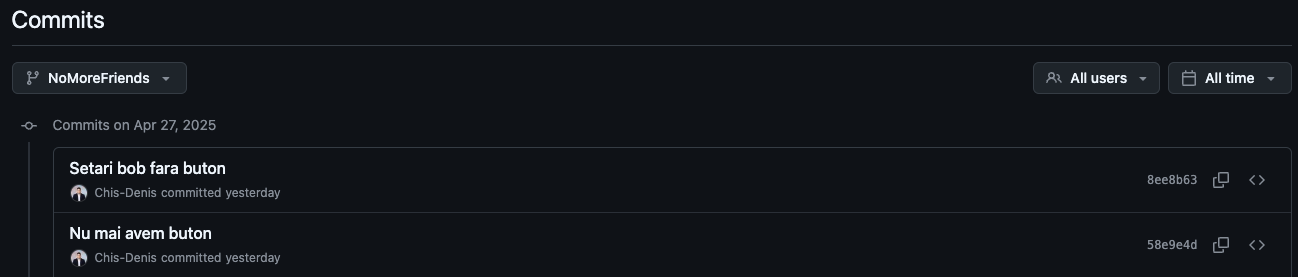
\includegraphics[width=0.9\columnwidth]{NoMoreFriends.png}
    \centering
    \caption{Branch "NoMoreFriends"}
    \end{figure}
    \item Branch \textbf{RefactorUserRepo} - 3 commits, authored by \textit{Tudor Buha}:
    \begin{figure}[H]
    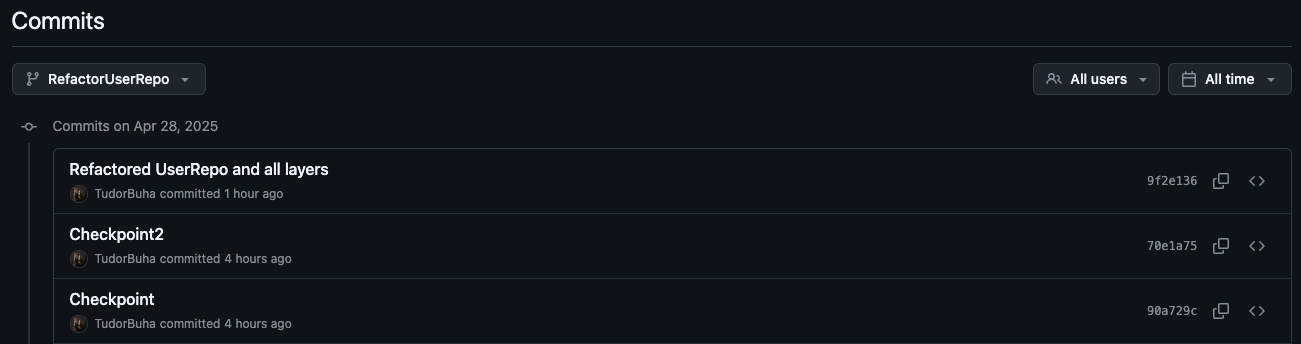
\includegraphics[width=0.9\columnwidth]{RefactorUserRepo.png}
    \centering
    \caption{Branch "RefactorUserRepo"}
    \end{figure}
    \item Branch \textbf{Robert/Hashtags2} - 5 commits, authored by \textit{Robert Bota}:
    \begin{figure}[H]
    \includegraphics[width=0.9\columnwidth]{Robert:Hashtags2.png}
    \centering
    \caption{Branch "Robert/Hashtags2"}
    \end{figure}
    \item Branch \textbf{Tudor} - 2 commits, authored by \textit{Tudor Buha}:
    \begin{figure}[H]
    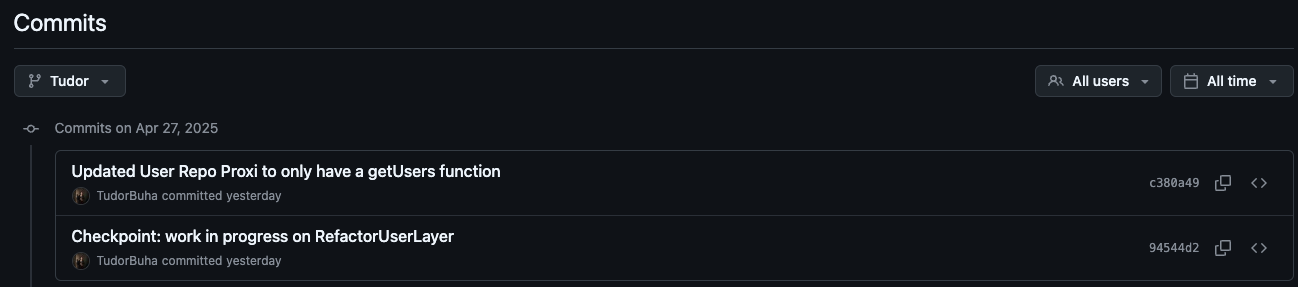
\includegraphics[width=0.9\columnwidth]{Tudor.png}
    \centering
    \caption{Branch "Tudor"}
    \end{figure}
    \item Branch \textbf{Vlad3} - 4 commits, authored by \textit{Vlad Cenușe}:
    \begin{figure}[H]
    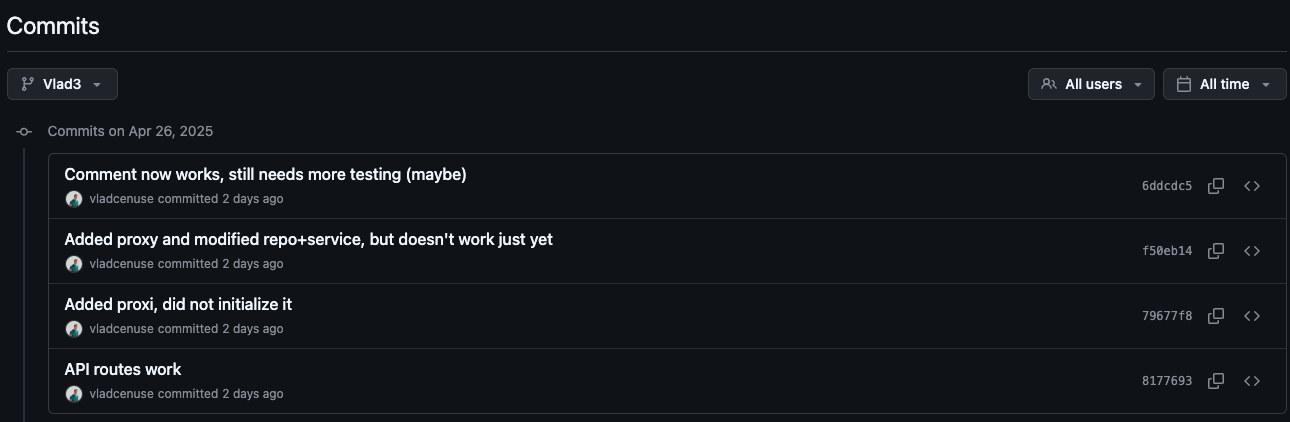
\includegraphics[width=0.9\columnwidth]{Vlad3.png}
    \centering
    \caption{Branch "Vlad3"}
    \end{figure}
    \item Branch \textbf{mihnea} - 5 commits, authored by \textit{Bota Mihnea} and \textit{Bogdan Borodi}:
    \begin{figure}[H]
    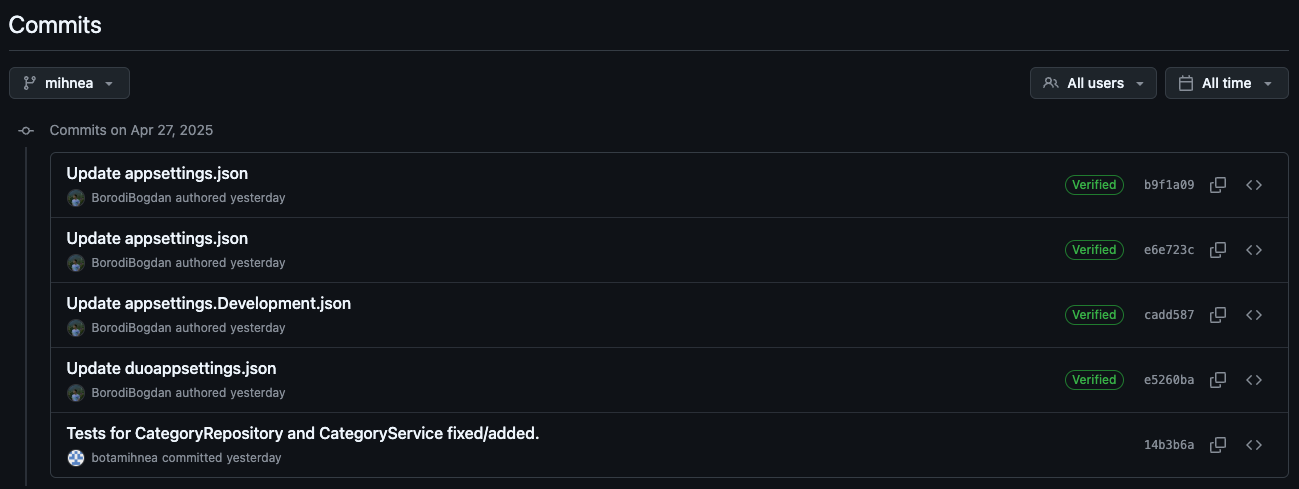
\includegraphics[width=0.9\columnwidth]{mihnea.png}
    \centering
    \caption{Branch "mihnea"}
    \end{figure}
    \item Branch \textbf{coty} - 11 commits, authored by \textit{Rareș Cotoi}, \textit{Bota Robert} and \textit{Bogdan Borodi}:
    \begin{figure}[H]
    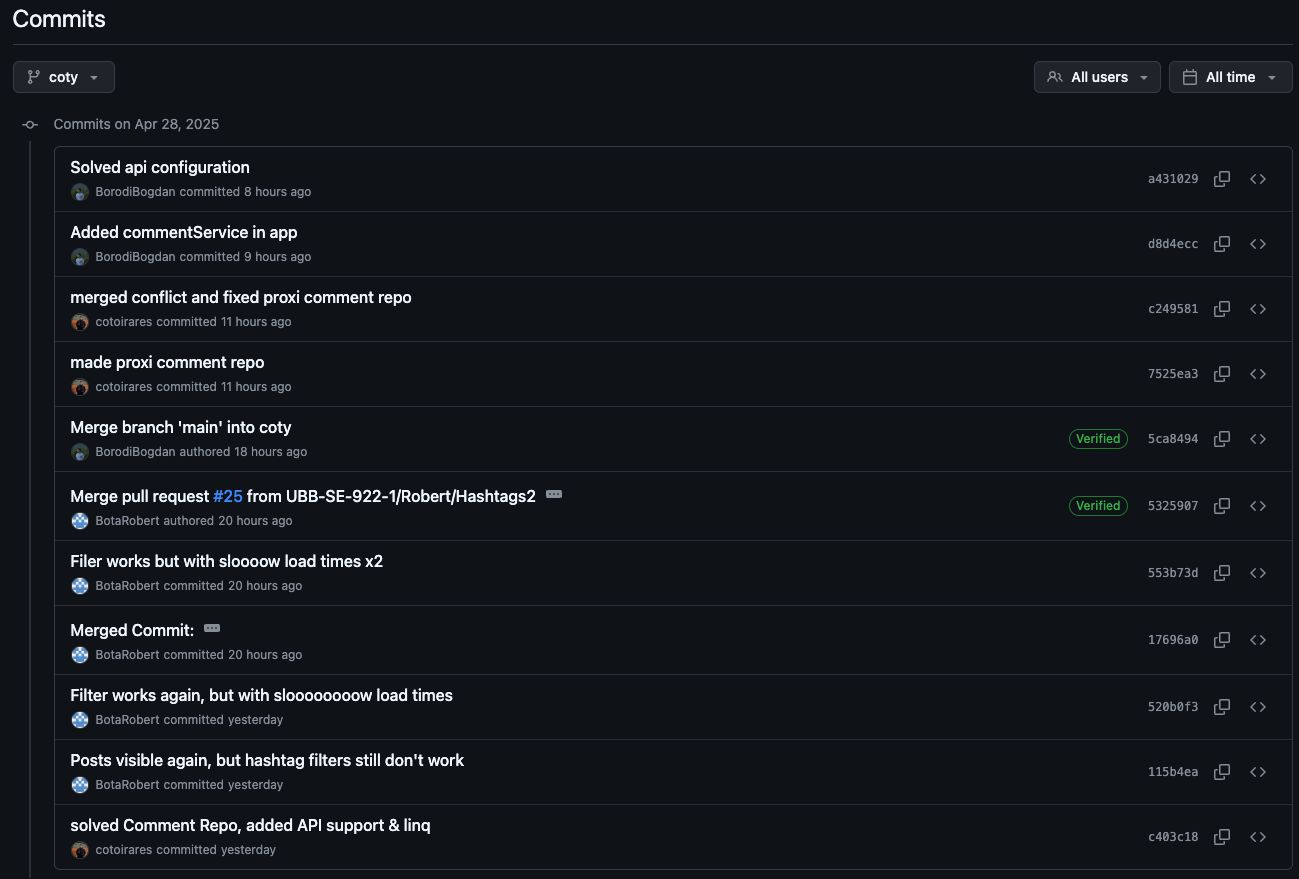
\includegraphics[width=0.9\columnwidth]{coty.png}
    \centering
    \caption{Branch "coty"}
    \end{figure}
\end{itemize}
    
\subsection{Lines of code contributed by each member}
For this Assignment, the total amount of contributed lines of code was \textbf{2470}. Please note that not all team members were assigned to contribute with lines of code.
    \begin{table}[H]
        \centering
        \caption{Lines of code contributed by each member}
        \label{tab:table}
        \begin{tabular}{ll}
            \toprule
            \textbf{Member} & \textbf{Lines contributed} \\
            \midrule
            Bogdan Borodi & 714 \\
            Vlad Cenușe & 472 \\
            Rareș Cotoi & 291 \\
            Robert Bota & 227 \\
            Tudor Buha & 182 \\
            Marian Chiticariu & 112 \\
            Mihnea Bota & 112 \\
            Denis Chiș & 109 \\
            Radu Cioată & 90 \\
            Cotîrlă Darius & 80 \\
            Teodora Buga & 54 \\
            Andrei Cruceru & 27\\
            \bottomrule   
        \end{tabular}
        
        \tabletext{Note: The total amount of contributed lines were calculated by iterating through each commit mentioned above.}
    \end{table}

\end{document}